% =====================================================================
\section{Special values, the golden comparison, and the OEIS
constellation}\label{sec:values}
% =====================================================================

Theorem~\ref{thm:transcendence} described the arithmetic of $\Tah(b)$
for rational $b$ in bulk; this section exhibits the concrete specimens.
Three families of exact values exist---integers, unit fractions, and
negative integers---and around them a constellation of five constants
has accumulated in the On-Line Encyclopedia of Integer Sequences, tied
together by elementary but pleasing identities.

\subsection{Exact values}

\begin{proposition}[exact values]\label{prop:exactvalues}
For every $n \in \N$,
\begin{equation}\label{eq:exact-families}
    \Tah\Bigl(\frac{n^{n}-1}{n}\Bigr) = n,
    \qquad
    \Tah\Bigl(n^{\,1-\frac{1}{n}} - n\Bigr) = \frac{1}{n} .
\end{equation}
The first family starts $0, \tfrac32, \tfrac{26}{3}, \tfrac{255}{4},
\tfrac{3124}{5},\ldots$ (at $x = 1,2,3,4,5,\ldots$); the second starts
$\sqrt2 - 2,\; 3^{2/3} - 3,\; 4^{3/4} - 4 = 2\sqrt2 - 4,\ldots$ (at
$x = \tfrac12, \tfrac13, \tfrac14, \ldots$). Together with
interpolation, these are the only rational arguments $b$ for which
$\Tah(b)$ is rational or algebraic (Theorem~\ref{thm:transcendence}).
\end{proposition}

\begin{proof}
Both identities are the statement $f(x) = b$ at $x = n$ and
$x = 1/n$: indeed $f(n) = (n^{n}-1)/n$, and
\[
    f\Bigl(\frac1n\Bigr) \;=\; \frac{(1/n)^{1/n} - 1}{1/n}
    \;=\; n \cdot \bigl(n^{-1/n} - 1\bigr)
    \;=\; n^{\,1-1/n} - n ,
\]
where $n^{\,1-1/n} = (n^{n-1})^{1/n}$ is the surd displayed. The
exactness was verified symbolically for $n \le 7$ and numerically to
eighty digits.
\end{proof}

The surd family gives $\Tah$ a supply of algebraic \emph{inputs} with
algebraic \emph{outputs}---$\Tah$ is not a transcendence machine
everywhere, only on the rational arguments off the two lattices
\eqref{eq:exact-families}. For instance
$\Tah(\sqrt2 - 2) = \tfrac12$ exactly, while $\Tah(-0.6)$, a
millimeter to the left on the $b$-axis, is transcendental.

\subsection{The golden comparison}

The quadratic pencil $x^{2} = bx + 1$ has positive root
$\varphi_b = (b + \sqrt{b^{2}+4})/2$, the family of metallic means
containing the golden ratio $\varphi = \varphi_1$. The super-quadratic
pencil has positive root $\Tah(b)$. The comparison between the two
turns out to be a \emph{single sign computation}.

\begin{theorem}[golden comparison]\label{thm:golden}
For all real $b$,
\[
\begin{aligned}
    \Tah(b) > \varphi_b \;&\iff\; 0 < b < \frac32,
    \qquad
    \Tah(b) = \varphi_b \iff b \in \Bigl\{0, \frac32\Bigr\},\\[1mm]
    \Tah(b) < \varphi_b \;&\iff\; b < 0 \text{ or } b > \frac32 .
\end{aligned}
\]
The two exact coincidences are $\Tah(0) = \varphi_{0} = 1$ and
$\Tah(\tfrac32) = \varphi_{3/2} = 2$.
\end{theorem}

\begin{proof}
Since $f$ is strictly increasing, $\Tah(b) > \varphi_b$ is equivalent
to $f(\varphi_b) < b$. But $\varphi_b$ solves $x^{2} = bx+1$, i.e.\
$b = \varphi_b - 1/\varphi_b$; therefore
\[
    f(\varphi_b) - b
    \;=\; \Bigl(\varphi_b^{\,\varphi_b - 1} - \frac{1}{\varphi_b}\Bigr)
    - \Bigl(\varphi_b - \frac{1}{\varphi_b}\Bigr)
    \;=\; \varphi_b^{\,\varphi_b - 1} - \varphi_b
    \;=\; \varphi_b \bigl(\varphi_b^{\,\varphi_b - 2} - 1\bigr),
\]
whose sign is the sign of $(\varphi_b - 2)\ln\varphi_b$. As
$b \mapsto \varphi_b$ is an increasing bijection $\R \to (0,\infty)$
with $\varphi_0 = 1$ and $\varphi_{3/2} = 2$, the sign is positive
exactly for $1 < \varphi_b < 2$, i.e.\ $0 < b < \tfrac32$, zero exactly
at $\varphi_b \in \{1,2\}$, and negative on the two outside intervals.
\end{proof}

\begin{remark}
The coincidence set $\{0, \tfrac32\}$ reflects the accident
$n^{n} = n^{2}$, which holds \emph{only} for $n \in \{1,2\}$: the
super-square and the square agree at $1$ and $2$ and nowhere else. It
is pleasant that the two most famous members of the two pencils---the
golden ratio and the Tahawus constant---obey
$\varphi < \alpha = \Tah(1) = 1.7767\ldots$, and that the ``excess''
$\Tah(b) - \varphi_b$, which vanishes at both ends of
$(0,\tfrac32)$, peaks at about $0.19000\ldots$ near $b \approx 0.7$
(between the rows $0.5$ and $1$ of Table~\ref{tab:golden}).
\end{remark}

\begin{table}[t]
\centering
\small
\caption{The Tahawus root versus the metallic root of the same
super-quadratic/quadratic $b$. The difference vanishes exactly at
$b = 0$ and $b = 3/2$ and changes sign there.}
\label{tab:golden}
\begin{tabular}{rrrr}
\toprule
$b$ & $\Tah(b)$ & $\varphi_b$ & $\Tah(b) - \varphi_b$ \\
\midrule
$-1$    & $0.3036591$  & $0.6180340$  & $-0.3143749$ \\
$-0.5$  & $0.5565737$  & $0.7807764$  & $-0.2242027$ \\
$0.5$   & $1.4559593$  & $1.2807764$  & $+0.1751828$ \\
$1$     & $1.7767750$  & $1.6180340$  & $+0.1587411$ \\
$1.4$   & $1.9609108$  & $1.9206556$  & $+0.0402552$ \\
$1.49$  & $1.9961956$  & $1.9920064$  & $+0.0041892$ \\
$1.5$   & $2.0000000$  & $2.0000000$  & $0$ \\
$1.51$  & $2.0037821$  & $2.0080064$  & $-0.0042243$ \\
$2$     & $2.1657594$  & $2.4142136$  & $-0.2484542$ \\
$3$     & $2.4019926$  & $3.3027756$  & $-0.9007830$ \\
$10$    & $3.0770622$  & $10.0990195$ & $-7.0219573$ \\
\bottomrule
\end{tabular}
\end{table}

\subsection{Negative integer roots, and the census of real roots}
\label{subsec:negative}

For negative $x$ the power $x^{x}$ is multivalued; we use the
principal branch $x^{x} = \exp(x \Log x)$, under which $x^{x}$ is real
precisely for negative integers (this is the branch plotted in
Figure~\ref{fig:slit}). The defining equation of the super-quadratic
then admits a second, exactly solvable family.

\begin{theorem}[negative integer roots]\label{thm:negroots}
\begin{enumerate}[label=\textup{(\roman*)}, leftmargin=2.4em]
\item For every $n \in \N$, the negative integer $x = -n$ solves
\[
    x^{x} \;=\; b_{n}\,x + 1
    \qquad\text{with}\qquad
    b_{n} \;:=\; \frac{1 - (-1)^{n}\, n^{-n}}{n} \;\in\; \Q ,
\]
e.g.\ $(-1)^{-1} = -1 = 2\cdot(-1) + 1$ (so $b_1 = 2$),
$(-2)^{-2} = \tfrac14 = \tfrac38 \cdot (-2) + 1$, and the sequence
$b_{n} = 2, \tfrac38, \tfrac{28}{81}, \tfrac{255}{1024}, \ldots$
alternates around $1/n$ and tends to $0$.
\item On the principal branch, $f(-r)$ is real \emph{if and only if}
$r \in \N$; hence the points \eqref{eq:bn-on-slit} are exactly the real
points of the slit $\gamma^{+} \cup \overline{\gamma^{+}}$ of
Figure~\ref{fig:slit}.
\item $\alpha$ is the unique \emph{real} root of $x^{x} = x + 1$ in
either convention for negative powers (principal branch, or the
real-branch convention $(-p/q)^{-p/q} := \bigl((-p/q)^{-p}\bigr)^{1/q}$
with $q$ odd).
\end{enumerate}
\end{theorem}

\begin{proof}
(i) $(-n)^{-n} = (-1)^{n} n^{-n}$, and
$(-1)^{n}n^{-n} = b_{n} \cdot (-n) + 1$ rearranges to
$b_{n} = (1 - (-1)^{n}n^{-n})/n$; these are rational, and the
identities were verified symbolically for $n \le 7$.

(ii) On the principal branch $(-r)^{-r} =
\exp\bigl(-r\ln r - i\pi r\bigr) = r^{-r}\ee^{-i\pi r}$, so
\[
    f(-r) \;=\; \frac{(-r)^{-r} - 1}{-r}
    \;=\; \frac{1 - r^{-r}\ee^{-i\pi r}}{r} ,
\]
which is real iff $\ee^{-i\pi r}$ is real, i.e.\ iff $\sin(\pi r) =
0$, i.e.\ iff $r \in \Z$; positivity of $r$ gives $r \in \N$. Then
\eqref{eq:bn-on-slit} applies.

(iii) On the principal branch, $x^{x} \in \R$ for $x < 0$ only at the
integers (part (ii)), and $x = -n$ solves $x^{x} = x + 1$ only if
$b_{n} = 1$, which never happens: $b_{1} = 2$, and for $n \ge 2$,
$b_{n} \le (1 + 2^{-2})/n \le \tfrac{5}{4}\cdot\tfrac12 < 1$. Under
the real-branch convention, a negative candidate is $x = -p/q$ in
lowest terms with $q$ odd. If $q \ge 2$, then
$x^{x} = (-1)^{p} (q/p)^{p/q}$ is \emph{irrational}: were
$(q/p)^{p/q} = m/n$ rational, raising to the $q$-th power would give
$q^{p} n^{q} = m^{q} p^{p}$, and the valuation argument of
Lemma~\ref{lem:irrational} applied with $p$ and $q$ interchanged (any
prime divisor $\ell$ of $q$ divides neither $p$ nor $m^{q}$'s factor,
forcing $q \mid v_\ell(q) \le \log_{2} q < q$, a contradiction)
rules this out. An irrational left-hand side cannot equal the rational
$x + 1$, so no $q \ge 2$ works; $q = 1$ returns to the integers,
already excluded. Hence the only real root of $x^{x} = x+1$ is the
positive one, $\alpha$.
\end{proof}

\subsection{The constellation of constants}\label{subsec:network}

Around $\alpha$ and $\beta = \Tah(-1)$ there orbits a small family of
constants, all present in the OEIS, all transcendental, and all
connected by elementary transformations. Recall
$\beta^{\beta} + \beta = 1$ and put
\[
    c \;:=\; \frac{1}{\beta} \;=\; 3.2931662874118610\ldots,
    \qquad
    v \;:=\; c - 1 \;=\; \frac{1}{\beta} - 1 \;=\;
    2.2931662874118610\ldots
\]

\begin{theorem}[the constellation]\label{thm:network}
\begin{enumerate}[label=\textup{(\roman*)}, leftmargin=2.4em]
\item The following are equivalent for $v > 0$ (and all hold for
$v = 1/\beta - 1$):
\[
    v^{\,1+1/v} = v + 1
    \;\iff\; v = \Bigl(1+\frac1v\Bigr)^{v}
    \;\iff\; v^{\,1/v} = (v+1)^{\,1/(v+1)}
    \;\iff\; v^{v+1} = (v+1)^{v} .
\]
\item $c = v + 1$ satisfies $c^{\,c-1} = (c-1)^{c}$, equivalently
$\frac{\ln c}{c} = \frac{\ln(c-1)}{c-1}$; this equation has a unique
real solution, lying in $(\ee, \ee+1)$.
\item The equation $v^{\,1/v} = (v+1)^{\,1/(v+1)}$ has the unique
solution $v \in (1, \ee)$ above: $v$ and $v+1$ are the unique pair of
\emph{consecutive} positive reals with equal $x^{1/x}$, the analogue
for $x^{1/x}$ of the classical pair $(2,4)$.
\item For each integer $k \ge 1$ the equation
$x^{\,1+1/x} = x + k$ has a unique positive solution
$\upsilon_k > 1$; $\upsilon_1 = v$ and
\[
    \upsilon_2 \;=\; 5.5079856527731782575890\ldots
    \qquad (\textrm{A144184}) .
\]
\item All five constants $\alpha$ (A124930), $\beta$ (A226568),
$c = 1/\beta$ (A169862), $v = c - 1$ (A085846) and $\upsilon_2$
(A144184) are transcendental.
\end{enumerate}
\end{theorem}

\begin{proof}
(i) $v^{\,1+1/v} = v + 1$ says $v \cdot v^{1/v} = v+1$, i.e.\
$v^{1/v} = (v+1)/v = 1 + 1/v$; raising both sides to the power $v$
gives $v = (1+1/v)^{v}$. Next, $v^{1/v} = (v+1)^{1/(v+1)}$ raised to
the power $v(v+1)$ gives $v^{v+1} = (v+1)^{v}$, and dividing the
exponents by $v(v+1)$ returns the equality of the $1/x$-powers; and
$v^{v+1} = (v+1)^{v}$ divided by $v^{v}$ is $v = ((v+1)/v)^{v} =
(1+1/v)^{v}$. For the bridge from $\beta$: $\beta^{\beta} = 1-\beta$
with $\beta = 1/c$ reads $(1/c)^{1/c} = (c-1)/c$; raising to the power
$c$ gives $1/c = (c-1)^{c}/c^{c}$, i.e.\ $c^{c-1} = (c-1)^{c}$, which
is (ii) for $c$, and it translates to $v^{1/v} = (v+1)^{1/(v+1)}$ by
taking $c = v+1$ and dividing exponents by $c(c-1)$.

(ii) The function $\ln x / x$ increases on $(0,\ee)$ and decreases on
$(\ee,\infty)$; thus $\ln c/c = \ln(c-1)/(c-1)$ forces $c - 1 < \ee <
c$, i.e.\ $c \in (\ee, \ee+1)$, and on this interval the difference
$\ln x/x - \ln(x-1)/(x-1)$ is strictly decreasing (its first term
decreases, its second increases), vanishing at most once; it vanishes
at $c = 1/\beta$ by the computation above.

(iii) is (ii) restated at $x = v + 1$: the pairs $x, x+1$ with equal
$x^{1/x}$ correspond exactly to $c = x+1$ solving (ii), and
$x = v \in (1, \ee)$.

(iv) Put $\psi(x) := x^{1+1/x} - x = x\bigl(x^{1/x} - 1\bigr)$. Then
$\psi(1) = 0$, and $\psi$ is strictly increasing on $[1, \infty)$:
indeed, with $L := \ln x \ge 0$,
\[
    x^{1/x - 1}\bigl(x + 1 - L\bigr)
    \;=\; \frac{x^{1/x}}{x}\bigl(x + 1 - L\bigr)
    \;\ge\; \Bigl(1 + \frac{L}{x}\Bigr)\frac{x + 1 - L}{x}
    \;=\; \frac{(x + L)(x + 1 - L)}{x^{2}}
    \;>\; 1 ,
\]
the last step because $(x+L)(x+1-L) = x^{2} + x + L - L^{2} > x^{2}$,
owing to $x > L^{2} - L$, which follows from $L^{2} < x$
(Lemma~\ref{lem:logsquare}); and the chain says exactly that
$\psi'(x) = x^{1+1/x}\bigl(x+1-\ln x\bigr)/x^{2} - 1 > 0$. Since
$\psi(1) = 0$ and $\psi(x) \to \infty$ (as $x^{1/x} \to 1$ and
$x \to \infty$), each value $k > 0$ is taken exactly once. The value
of $\upsilon_2$ was located numerically and its equation verified.

(v) $\alpha$ and $\beta$ are transcendental by
Corollary~\ref{cor:stanley}; $c$ and $v$ are nonconstant rational
functions of $\beta$, hence transcendental. For $\upsilon_2 =: w$: if
$w$ were algebraic irrational, then $w \notin \{0,1\}$ and
$w^{1/w}$ would be transcendental by Gelfond--Schneider, making
$w^{\,1+1/w} = w \cdot w^{1/w}$ transcendental---contradicting
$w^{\,1+1/w} = w + 2$ algebraic. If $w = p/q$ were rational (lowest
terms), raising $ (p/q)^{1+q/p} = (p+2q)/q$ to the $p$-th power gives
\[
    p^{\,p+q} \;=\; (p+2q)^{p}\, q^{\,q} .
\]
Any odd prime $\ell \mid p$ divides neither $q$ nor $p + 2q$ (since
$\gcd(p, p+2q)$ divides $2$), so comparing $v_\ell$ on both sides gives
$(p+q)\,v_\ell(p) = 0$, impossible; hence $p = 2^{a}$. If $a \ge 2$,
then $v_2(p+2q) = 1$ (as $2^{a-1} + q$ is odd) and $v_2$ gives
$a(p+q) = p$, impossible for $a \ge 2$. If $a = 1$, then $p = 2$ and
$v_2(2 + 2q) = 1 + v_2(1+q)$, so $(2+q) = 2(1 + v_2(1+q))$, forcing the
odd number $q$ to equal the even number $2\,v_2(1+q)$---impossible.
So $w$ is neither rational nor algebraic irrational.
\end{proof}

\begin{figure}[t]
    \centering
    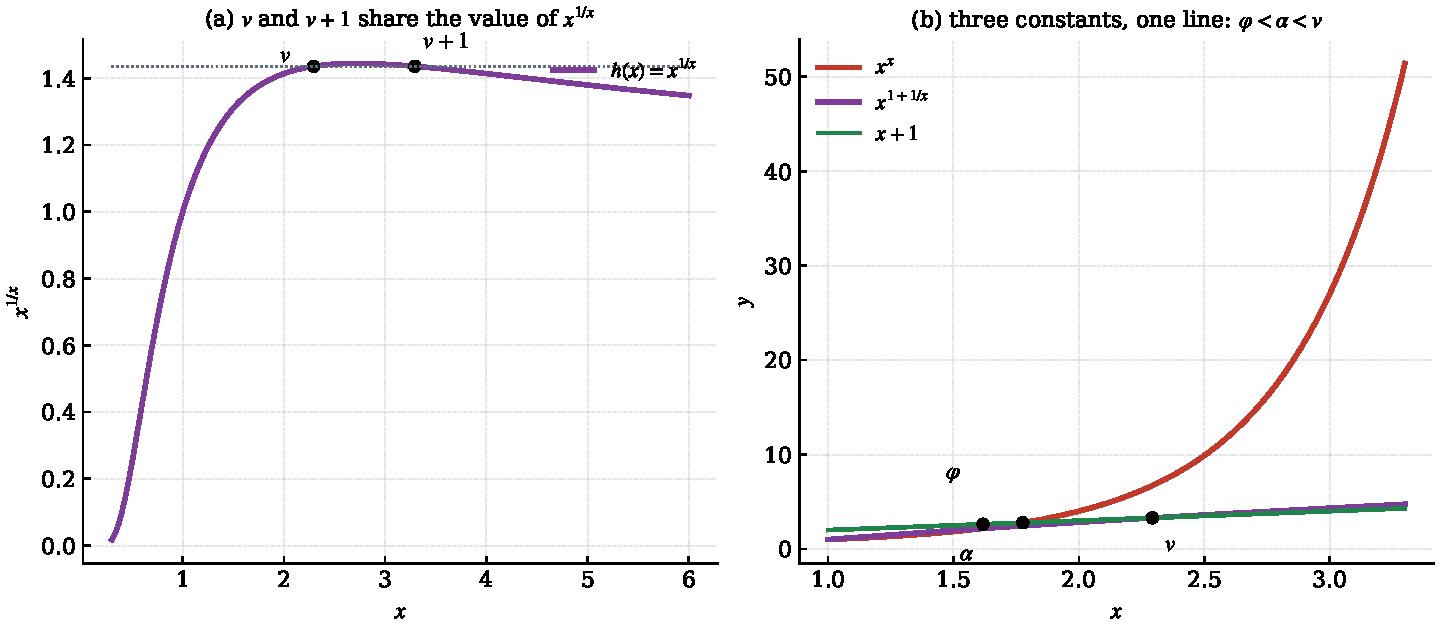
\includegraphics[width=0.98\textwidth]{figures/fig6_constants.pdf}
    \caption{(a) The map $h(x) = x^{1/x}$ is unimodal with maximum at
    $\ee$; the consecutive pair $v, v+1$ (marked, with the dotted level
    line) is the unique pair of consecutive reals on which $h$ takes
    equal values---for $h$, what the pair $(2,4)$ is classically.
    (b) The line $y = x+1$ (green), the curve $x^{x}$ (red) and the
    curve $x^{1+1/x}$ (purple): the two curves exchange order at
    $x = \varphi$ (where the exponents $x$ and $1+1/x$ coincide), the
    line is met by $x^{x}$ at $\alpha$ and by $x^{1+1/x}$ at $v$;
    consequently $\varphi < \alpha < v$, the three parameters marked
    at their heights on the line.}
    \label{fig:constants}
\end{figure}

\begin{remark}[credits and digit agreement]\label{rem:credits}
The five OEIS entries are A124930 ($\alpha$, root of $x^x = x+1$),
A226568 ($\beta$, ``the number defined by $x^x + x = 1$''), A169862
($c$, root of $x^{x-1} = (x-1)^x$), A085846 ($v$, root of
$x = (1+1/x)^x$) and A144184 ($\upsilon_2$, root of
$x^{1+1/x} = x+2$) \cite{a124930,a226568,a169862,a085846,a144184}.
Our independently computed decimal expansions of $\alpha$ and $v$ agree
digit for digit with the seventy-digit strings recorded in A124930 and
A085846, and $\beta$ agrees with the blog post's value
\cite{blog}; $c = v + 1$ and $\upsilon_2$ were verified through their
defining equations. Lord \cite{lord} proved the transcendence of $v$ by
the equivalent equation $x = (1+1/x)^{x}$; Theorem~\ref{thm:network}(v)
extends the pattern to the whole family $\upsilon_k$. The quantity
$\alpha^{\alpha-1} = 1 + 1/\alpha$ implicit in the figure, and the
identity $\beta^{\beta - 1} = (1-\beta)/\beta = v$, are the two edges
along which the constellation connects back to $\Tah$.
\end{remark}
